\documentclass[10pt,showpacs,preprintnumbers,amsmath,amssymb,nofootinbib,aps,prl,twocolumn,groupedaddress,superscriptaddress,showkeys]{revtex4-1}
\usepackage{graphicx}
\usepackage{subfig}
\usepackage[colorlinks=true,urlcolor=blue,citecolor=blue]{hyperref}
\usepackage{listings}
\usepackage{tikz} % Send help 
  \usetikzlibrary{automata, positioning}
\usepackage{physics}
%\usepackage{dcolumn}
%\usepackage{bm}
%\usepackage{color}
%\usepackage{float}

\lstset{ %
  basicstyle=\footnotesize,        % the size of the fonts that are used for the code
  breakatwhitespace=false,         % sets if automatic breaks should only happen at whitespace
  breaklines=true,                 % sets automatic line breaking
  captionpos=t,                    % sets the caption-position to bottom
  deletekeywords={...},            % if you want to delete keywords from the given language
  escapeinside={\%*}{*)},          % if you want to add LaTeX within your code
  extendedchars=true,              % lets you use non-ASCII characters; for 8-bits encodings only, does not work with UTF-8
  frame=single,                    % adds a frame around the code
  keepspaces=true,                 % keeps spaces in text, useful for keeping indentation of code (possibly needs columns=flexible)
 % language=Python,                 % the language of the coderevtex aps style
  morekeywords={*,...},           % if you want to add more keywords to the set
  numbers=left,                    % where to put the line-numbers; possible values are (none, left, right)
  numbersep=5pt,                   % how far the line-numbers are from the code
  showspaces=false,                % show spaces everywhere adding particular underscores; it overrides 'showstringspaces'
  showstringspaces=false,          % underline spaces within strings only
  showtabs=false,                  % show tabs within strings adding particular underscores
  stepnumber=1,                    % the step between two line-numbers. If it's 1, each line will be numbered
  tabsize=2,                       % sets default tabsize to 2 spaces
}

\captionsetup[subfigure]{labelformat=brace}

\begin{document}
\title{Disease Modeling - FYS3150 Computational Physics}
\author{Nicholas Karlsen}


\begin{abstract}
  This is an abstract
\end{abstract}

\maketitle


\section{Introduction}

\section{Theory, Algorithms and Methods}
  \subsection{SIRS Model}

    The SIRS model is a mathematical model from epidemiology describing how infectious disease evolves within a population, and is a part of a family of similar models in epidemiology with various different features. In the SIRS model, the total population (N) is divided into three groups

    \begin{itemize}
      \item Susceptible (S) : People who do not have the disease, and are not immune to it.
      \item Infected (I) : People who are infected with the disease.
      \item Recovered (R) : People who has recovered from the infection, and have developed immunity.
    \end{itemize}

    Where in the simplest case, the permitted traversal from one group to another follows a cyclical pattern $S \rightarrow I \rightarrow R \rightarrow S$, hence the name SIRS.

    The rate of traversal is governed by a set of coupled differential equations,

    \begin{align}
      \begin{split}
        S' &= cR - \frac{aSI}{N} \\
        I' &= \frac{aSI}{N} - bI \\
        R' &= bI - cR 
        \label{eqn:transition rates, basic}
      \end{split}
    \end{align}
    Where the constants $a,b,c$ are governing the

    \begin{itemize}
      \item rate of transmission
      \item rate of recovery
      \item rate of immunity loss
    \end{itemize}

    respectively, with dimension inverse time. For the purposes of this report, we will not consider any particular unit of time, but rather the dynamics of the system, as the timescales at which different diseases operate on vary. However, based on data (INSERT CITATIONS) a lot of common diseases are observed to operate on a scale of days, whilst some operate on a scale of years. 

    We note here that each term in the system of equations is reflected in opposite, for a different group. For example, the $cR$ term in $S'$ is mirrored in opposite in $R'$ as $-cR$. As defined earlier, $c$ denotes the rate of immunity loss, so these terms essentially moves people in the R group to the S group.
    The result of this is that that the total population is conserved in this system, such that we have a constant $N = S(t) + I(t) + R(t)$.

    As shown in \textcite{project5}, we can then substitute this into the set of equations \ref{eqn:transition rates, basic} and derive equations for how the system distributes itself in a steady state

    \begin{align}
      \begin{split}
        s^* &= \frac{b}{a}  \\
        i^* &= \frac{1 - \frac{b}{a}}{1 + {b}{c}} \\
        r^* &= \frac{b}{c}\frac{1 - \frac{b}{a}}{1 + \frac{b}{c}}
      \end{split}
    \end{align}

    which notably only depends upon the parameters governing the system. Meaning that for some set of parameters, $a,b,c$ the system will always converge towards the same state given enough time. Matching the behaviour of what we expect from a Markov chain governed by a regular stochastic matrix as shown in for example, \textcite[p.~277, theorem~18]{linalg_lays}.

    \begin{figure}[h!tbp]
      \centering 
      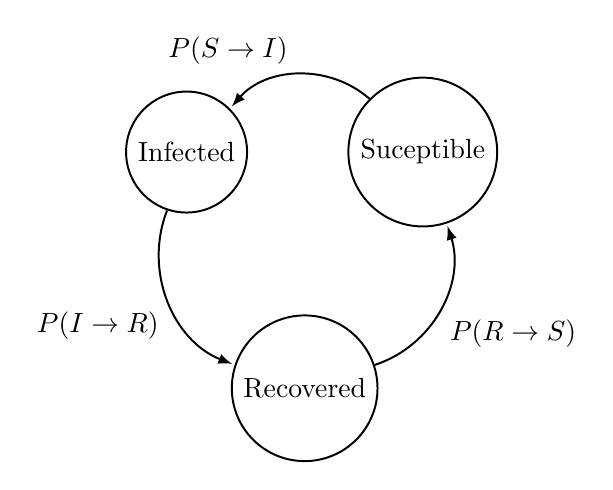
\begin{tikzpicture}
 
        % Setup the style for the states
        \tikzset{node style/.style={state, 
                                    minimum width=1.5cm,
                                    line width=.25mm
                                    }}
 
        % Draw the states
        \node[node style] at (3, 0)     (Suceptible)     {Suceptible};
        \node[node style] at (0, 0)     (Infected)     {Infected};
        \node[node style] at (1.5, -3) (Recovered) {Recovered};
 
        % Connect the states with arrows
        \draw[every loop,
              auto=right,
              line width=.25mm,
              >=latex]
            (Suceptible)    edge[bend right=45]  node {$P(S\rightarrow I)$} (Infected)
            (Infected)      edge[bend right=45]  node {$P(I\rightarrow R)$} (Recovered)
            (Recovered)     edge[bend right=45]  node {$P(R\rightarrow S)$} (Suceptible);
      \end{tikzpicture}
       \caption{Markov diagram for the basic SIRS model\label{fig:SIRS diagram}}
    \end{figure}

    \subsubsection{Extending the SIRS model}
      The model described by Eqn.\ref{eqn:transition rates, basic}, henceforth referred to as the Basic SIRS model can be extended to model other behaviours relevant to the study of an illness. In this project, we will specifically look at 3 extensions to the model, that is: Vital dynamics, Seasonal variation and vaccinations.

      Starting off, we add the effect of vital dynamics to our set of differential equations in the following way

      \begin{align}
        \begin{split}
          S' &= cR - \frac{aSI}{N} - dS\\
          I' &= \frac{aSI}{N} - bI - (d + d_I)I \\
          R' &= bI - cR - dR
        \label{eqn:transition rates, vitdyn}
      \end{split}
    \end{align}

    where $d$ denotes the death rate of the population, and $d_I$ the added death rate of the Infected group of the population. We see here that the new terms are not mirrored in the same way as that constitute the basic model such that the system is generally speaking no longer population conservative if any of these terms are non-zero. With a possible exception being for example if $d=0,\enspace a=0,\enspace d_I>0$ and $I_0 = 0$, in which case the population would be conserved.


    Seasonal variation, or simply a periodic behaviour in the rate of transmission, added to the model by no longer having a constant $a$, but instead letting it be a function of time as
    \begin{equation}
      a(t) = A\cos(\omega t) + a_0
      \label{eqn: seavar}
    \end{equation}

    Where $a_0$ denotes the baseline rate of transmission, $A$ the maximum deviation from the baseline and $\omega$ the frequency of the variation. 

    and lastly, we look at a possible way modelling the effects of vaccinations by this time adding a term $f$, denoting the rate of vaccination to our basic model in the following way

    \begin{align}
        \begin{split}
          S' &= cR - \frac{aSI}{N} - f\\
          I' &= \frac{aSI}{N} - bI\\
          R' &= bI - cR + f
        \label{eqn:transition rates, vaxx}
      \end{split}
    \end{align}

    We see here that this addition of this terms allows someone in the S group to go immediately to the I group, which as intended. Further, this transition rate from $S\rightarrow I$ is not dependent on the population, or size of any population groups unlike any of the other behaviours modelled thus far. Whilst we will save the discussion on the many implications this has later, we note here a particular, significant flaw in this extension to the model. Whilst it is still population conservative if we look only at $N = S(t) + I(t) + R(t)$, it does present the possibility of $S(t)<0$, which is entirely un-realistic.


  \subsection{Monte-Carlo Algorithm}
    We will now build a Monte-Carlo algorithm for simulating the dynamics of disease modelled by the different sets of equations we have looked at. These simulations aims to, on average match the behaviour predicted by the differential equations, but in a more realistic way by first and foremost allowing only discrete, transitions from from one group to another instead of continuous ones. And further, imposing certain restrictions to prevent unintended behaviours such as any of the groups becoming negative, which as mentioned earlier is a possibility in the system modelling the effects of vaccinations, in Eqn. \ref{eqn:transition rates, vaxx}.

    In \textcite{project5} we are methodology of translating the sets of differential equations to a set of transition probabilities for the basic model
    \begin{align}
      \begin{split}
        P(S\rightarrow I) &= \frac{aSI}{N}\Delta t \\
        P(I\rightarrow R) &= bI\Delta t \\
        P(R\rightarrow S) &= cR\Delta t
        \label{eqn:basic probabilities}
      \end{split}
    \end{align}

    and a step-size
    \begin{equation}
      \Delta t = \text{min}\left\{ \frac{4}{aN}, \frac{1}{bN}, \frac{1}{cN} \right\}
      \label{enq:basic dt}
    \end{equation}

     where for each step we evaluate the transition probabilities against a random number $r\in[0,1]$. If the transition probability is greater than $r$, the transition is made, else, it isn't. This constitutes the Monte-Carlo part of the algorithm, and in order to produce expectation values we take the average of many cycles of systems initiated in the same way, and evolved following these rules. 

     Shown below in Pseudo-code
\begin{lstlisting}[mathescape=true, language=python, title=SIRS Monte-Carlo]
for each $\textbf{MC-Cycle}$:
  for each $t_i$:
    Compute $P(S\rightarrow I)$
    Compute $P(I\rightarrow R)$
    Compute $P(R\rightarrow S)$

    if $P(S\rightarrow I)> r$ and $S_i > 0$:
      $S_{i+1}$ -= 1
      $I_{i+1}$ += 1

    if $P(I\rightarrow R)> r$ and $I_i > 0$:
      $I_{i+1}$ -= 1
      $R_{i+1}$ += 1

    if $P(R\rightarrow S)> r$ and $R_i > 0$:
      $R_{i+1}$ -= 1
      $S_{i+1}$ += 1
\end{lstlisting}
  
  Extending algorithm for the model extensions to the basic model is done quite easily by following the same logic outlined in \textcite{project5}. If we consider the system the addition of vital dynamics, we have three additional permitted transitions, one for each group. $S\rightarrow DEAD$, $I\rightarrow DEAD$ and $R \rightarrow DEAD$. The transition probabilities for each time-step is then given by
  \begin{align}
    \begin{split}
      P(S\rightarrow DEAD) &= dS \Delta t \\
      P(I\rightarrow DEAD) &= (d + d_I)I\Delta t \\ 
      P(R\rightarrow DEAD) &= dR\Delta t
    \end{split}
  \end{align}

  where the time step is now given by
  \begin{equation}
      \Delta t = \text{min}\left\{ \frac{4}{aN}, \frac{1}{bN}, \frac{1}{cN}, \frac{1}{dN}, \frac{1}{(d + d_I)N} \right\}
  \end{equation}

  Where the last entry of the set, $\frac{1}{(d+d_I)N}$ can be omitted for a slight performance increase as it will always be greater than $\frac{1}{dN}$.

  Out of the 4 variations of the SIRS model discussed in this project, this model in particular requires some extra attention, as the step size is a will vary differently in each Monte-Carlo cycle as the step size is dependent on N. This means, that when computing the expected path produced by multiple cycles of the Monte-Carlo algorithm, we interpolate between points to produce averages for some selection of times.


  \subsection{4th-order Runge-Kutta method}
    The 4th-order Runge-Kutta (RK4) is one part, of a family of methods for solving ordinary differential equations (ODE). In short, the Runge-Kutta methods consists of taking a weighted average of different finite-steps, in particular, for RK4 we have the steps

    \begin{align}
      \begin{split}
        \centering           
        k_1 &= f(t_i, y_i) \\
        k_2 &= f \qty(t_i + \frac{h}{2}, y_i + \frac{h}{2} \cdot k_1) \\
        k_3 &= f \qty(t_i + \frac{h}{2}, y_i + \frac{h}{2} \cdot k_2) \\
        k_4 &= f \qty(t_i + h, y_i + h\cdot k_3)
      \end{split}         
    \end{align}

    where $h$ denotes the step-size. A weighted average of these steps are then used to compute the $i+1$'th element in the following way.
    \begin{equation}
      y_{i+1} = y_i + \frac{1}{6}h\qty(k_1 + 2k_2 + 2k_3 + k_4) + \mathcal O(h^5)
    \end{equation}

    where $\mathcal O(h^5)$ is the error in this single step, and the a global error of $\mathcal O (h^4)$. For more details, refer to \textcite[p.~250]{compphys_lecnotes}.

\begin{figure*}[h!tb]
  \centering
  \subfloat[][]{
\includegraphics[height=0.75cm]{figs/prob_ab_legend.pdf}} \\
  \subfloat[][]{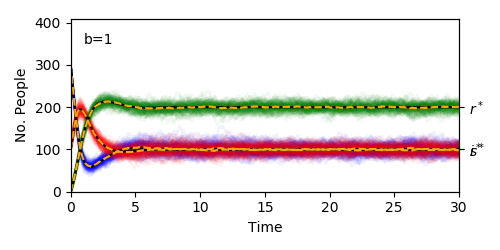
\includegraphics[width=8cm]{figs/prob_b_varb_1.png}}
  \subfloat[][]{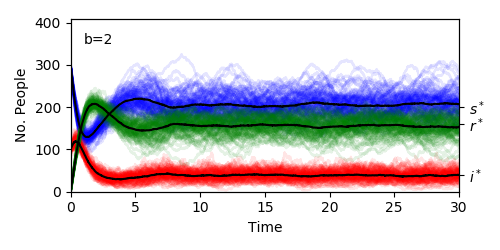
\includegraphics[width=8cm]{figs/prob_b_varb_2.png}} \\
  \subfloat[][]{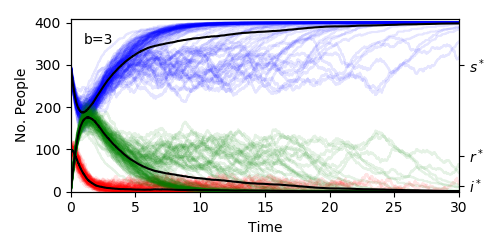
\includegraphics[width=8cm]{figs/prob_b_varb_3.png}}
  \subfloat[][]{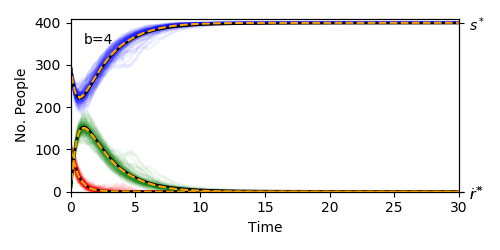
\includegraphics[width=8cm]{figs/prob_b_varb_4.png}}
  \caption{\label{fig:ab_plots}The basic SIRS model simulated by the Monte-Carlo simulation for 100 cycles, as well as the ODE solutions with initial state $S_0 = 300, I_0 = 100, R_0 = 0$, constants $a=4, c=0.5$ and $b=1,2,3,4$.}
\end{figure*}

\begin{figure*}[h!tb]
  \centering
  \subfloat[][]{
\includegraphics[height=0.75cm]{figs/prob_b_std_legend.pdf}} \\
  \subfloat[][]{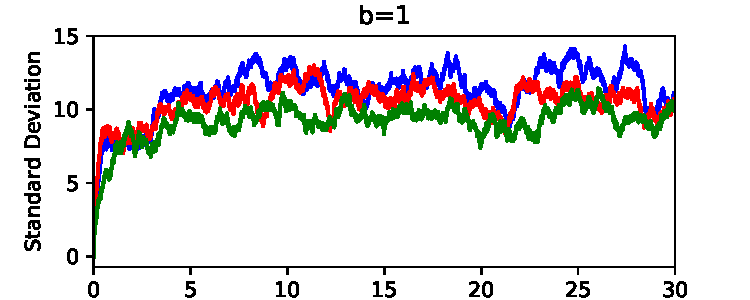
\includegraphics[width=8cm]{figs/prob_b_std_1.pdf}}
  \subfloat[][]{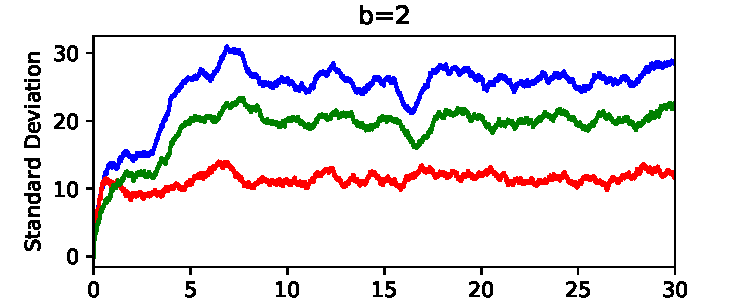
\includegraphics[width=8cm]{figs/prob_b_std_2.pdf}} \\
  \subfloat[][]{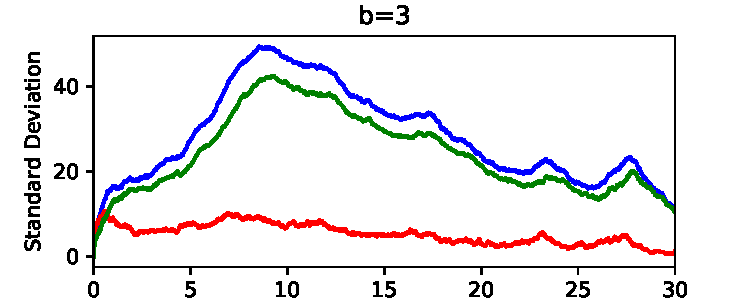
\includegraphics[width=8cm]{figs/prob_b_std_3.pdf}}
  \subfloat[][]{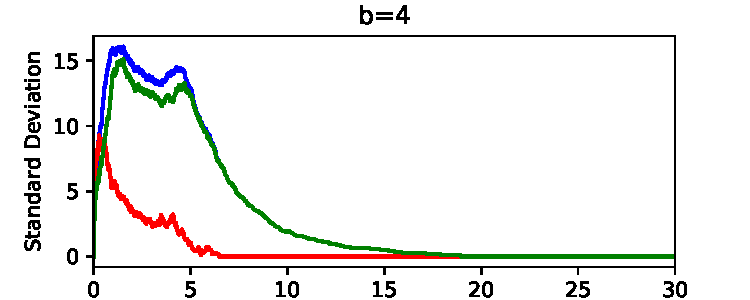
\includegraphics[width=8cm]{figs/prob_b_std_4.pdf}}
  \caption{\label{fig:standard deviations b}The standard deviations for each $b$ in the Monte Carlo solutions shown in Fig.~\ref{fig:ab_plots}, consisting of 100 cycles each.}
\end{figure*}

\begin{figure*}[h!tb]
  \subfloat[][]{
\includegraphics[width=8cm]{figs/prob_ab_legend.pdf}}
  \\
  \subfloat[][]{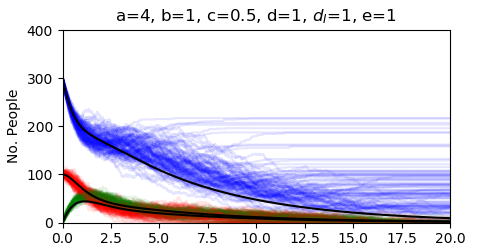
\includegraphics[width=8cm]{figs/prob_c_fig_0.png}}   
  \subfloat[][]{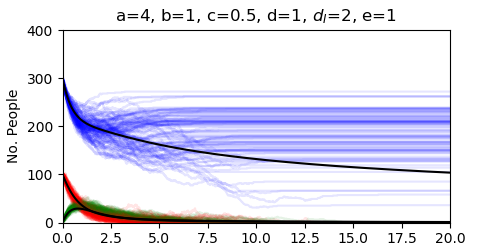
\includegraphics[width=8cm]{figs/prob_c_fig_1.png}}\\
  \subfloat[][]{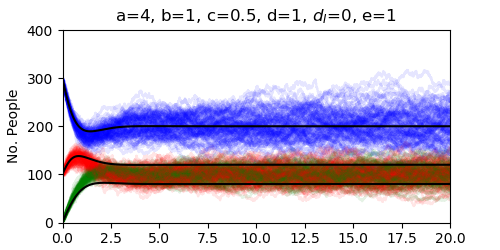
\includegraphics[width=8cm]{figs/prob_c_fig_2.png}\label{fig:c d=1 ,dI=1, e=1}}   
  \subfloat[][]{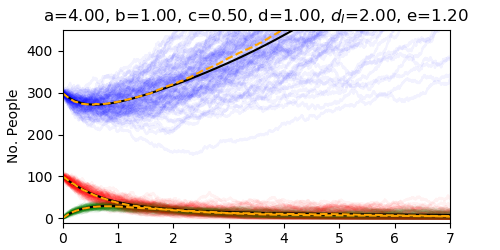
\includegraphics[width=8cm]{figs/prob_c_fig_3.png}}   
  \caption{\label{fig:prob c}The SIRS model with vital dynamics for initial state $S_0=300, I_0=100, R_0=0$ and constants $a=4, b=1, c=0.5$, and 100 MC cycles.}
\end{figure*}

\begin{figure*}[h!tb]
  \subfloat{
\includegraphics[width=8cm]{figs/prob_ab_legend.pdf}}
  \\
  \subfloat{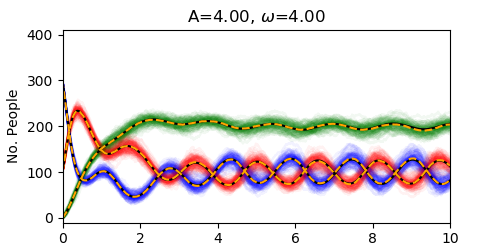
\includegraphics[width=8cm]{figs/prob_d_fig_0.png}}   
  \subfloat{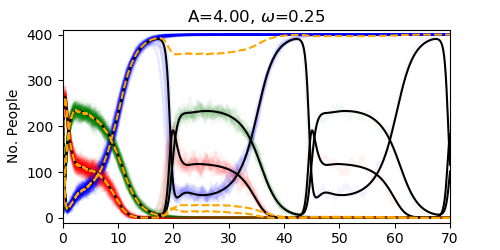
\includegraphics[width=8cm]{figs/prob_d_fig_1.png}}\\
  \subfloat{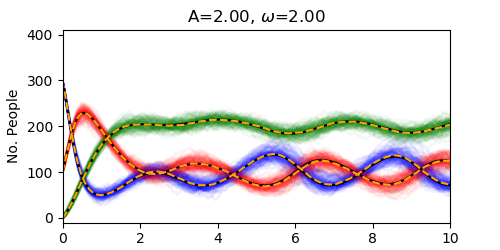
\includegraphics[width=8cm]{figs/prob_d_fig_2.png}}   
  \subfloat{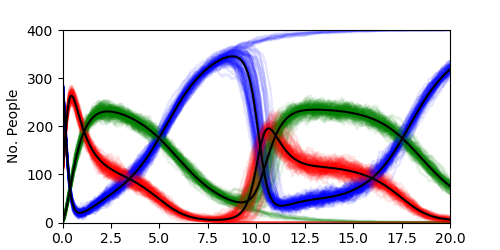
\includegraphics[width=8cm]{figs/prob_d_fig_3.png}}   
  \caption{\label{fig:prob d}The SIRS model with seasonal variation for initial state $S_0=300, I_0=100, R_0=0$ and constants $a=4, b=1, c=0.5$, and 100 MC cycles.}
\end{figure*}

\begin{figure*}[h!tb]
  \subfloat[][]{
\includegraphics[width=8cm]{figs/prob_ab_legend.pdf}}
  \\
  \subfloat[][]{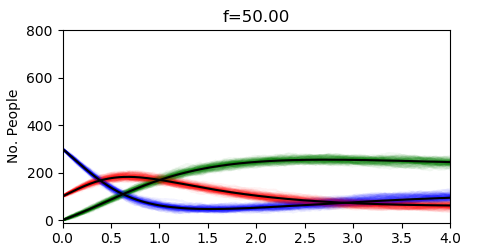
\includegraphics[width=8cm]{figs/prob_e_fig_0.png}}   
  \subfloat[][]{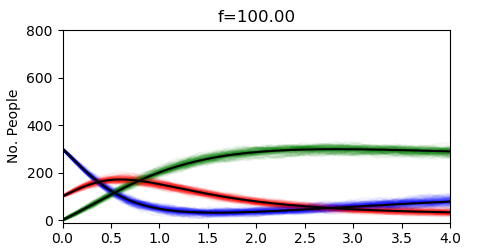
\includegraphics[width=8cm]{figs/prob_e_fig_1.png}}\\
  \subfloat[][]{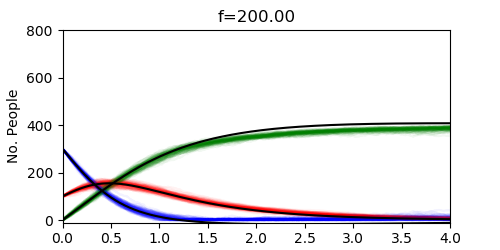
\includegraphics[width=8cm]{figs/prob_e_fig_2.png}}   
  \subfloat[][]{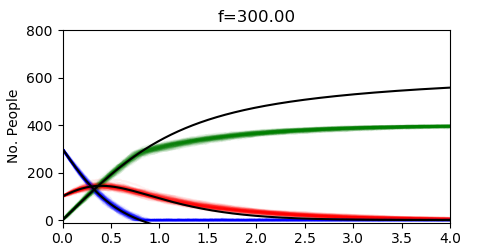
\includegraphics[width=8cm]{figs/prob_e_fig_3.png}\label{fig:c mc improvement}}   
  \caption{\label{fig:prob e}The SIRS model with vaccinations for initial state $S_0=300, I_0=100, R_0=0$ and constants $a_0=4, b=1, c=0.5$, and 100 MC cycles}
\end{figure*}

\section{Results and Discussions}
  \subsection{Implementation}
    Before we look at the results, i would like to make a quick remark in regards to the code, and its structure. My initial plan was to implement the entirety of the project in python, however, upon starting to consider how i might implement the vital dynamics, with its dynamic step sizes i decided to implement this, and the subsequent models in Julia\footnote{This also meant that i had to learn Julia, having only a "hello world"-level of understanding prior to this project.}, which generally speaking is much faster than pure python. A particular benefit of Julia being that there exists APIs that lets us call Julia functions directly from python, and in reverse. These APIs allowed me to very easily offload the heavier Monte-Carlo simulations to Julia, then performing the subsequent plotting and analysis in python. 

  \subsection{SIRS: Basic model}
    We start by looking at the results produced by both the RK4 solution to Eqn.~\ref{eqn:transition rates, basic} as well as the Monte-Carlo results for this system, for 100 cycles. The results are presented in a quite compact form in Fig.~\ref{fig:ab_plots}, where all 4 sub-plots share a common legend. In this, and subsequent plots the colours blue, red and green indicate the S, I and R groups respectively and individual MC cycles are plotted with a transparency of 5\%, such that common paths will display a greater hue than less common ones. Overlaid on top of these individual MC cycles are the ODE result, as well as the Mean Monte-Carlo result. For the sake of readability the Mean and ODE results have not been colour coded with individual colours for each group, but their belonging should be quite clear from the individual cycles on which they overlay.


    In these plots, the system was initiated in in the state $S_0 = 300, I_0=100$ and $R_0=0$ and the parameters $a=4, c=0.5$ are held constant throughout all 4 sets of data. We see that for the MC simulations, only 3 out of the 4 cases converges towards the predicted set of steady states, indicated by axis ticks on the right x-axes. In the case of $b=3$, we observe that neither the S or R groups converge towards their respective steady states. To investigate this further, we then refer to Fig.~\ref{fig:standard deviations b}, where we note how the standard deviation of the MC results seem to rise towards a peak from the beginning, until $t\approx10$, before it drops. To make sense as to why there is such a great uncertainty in this area, we refer to $b=1$ and $b=2$. We observe that the standard deviation in all 3 groups are quite consistent for $b=1$, then looking at the standard deviation for $b=2$  we see that standard deviation for the I group is similar to $b=1$, but the $R$, and particularly S group has a significantly higher standard deviation. We observe here, what I believe to be the main cause of uncertainty, and deviance from the ODE solution for the Monte-Algorithm. That is, whenever one (or more) of the groups tends towards either the upper or lower population limits, the uncertainty of the others seem to rise locally, and this error is then propagated forwards in time, even though the standard deviation in the MC simulations goes down again. We will investigate this hypothesis more thoroughly later in the model including seasonal variation, but for now we note that the uncertainty, and deviation from the ODE in the MC solutions isn't necessarily tied to the number of MC cycles, but the way in which the system evolves, and that we need to take into account the paths of each set of MC simulations when assessing any errors on a per-simulation basis rather than a per-system or per-number of iterations basis as is often the case in numerical methods\footnote{At least in my own, limited experience.}

    ADD CONVERGENCE CHECK FOR B=3


  \subsection{SIRS: Vital Dynamics}
    If we now turn to Fig.~\ref{fig:prob c} we see the plots for the vital dynamics system.
    For this model, we observe that the MC mean path follows mostly the ODE solution, deviating the most in Fig.~\ref{fig:c d=1 ,dI=1, e=1}, which out of the four data sets ends up hoovering the most around the lower-limit of the permitted group sizes.

    In a qualitative sense, we observe that the system is particularly sensitive to an increase in the birth rate, which very quickly dominates over the death rate. What's also interesting, is that in a growing population, a highly deadly disease may be short-lived in this in this model.

  \subsection{SIRS: Seasonal Variation}
    In Fig.~\ref{fig:prob d}, we see results that are somewhat similar to what we saw in the basic SIRS model, but instead of converging towards a constant steady state, the system instead tends towards a periodic steady state. We see also that the frequency $\omega$ plays into the amplitude of the variation within the groups in their steady state just as much, if not more than $A$. We also observe that there seems to be a natural frequency, in which we get a peak variation within groups once the steady state has been reached and we effectively observe a resonance\footnote{There should be a .gif showing this quite clearly in the README.md file in the main directory for this project.}. 

  \subsection{SIRS: Vaccinations}
    Finally, we turn to Fig.~\ref{fig:prob e}. Here we again see mostly good agreement between the MC and ODE results, except in Fig.~\ref{fig:c mc improvement}, which exemplifies how MC simulations may improve upon the systems of differential equations which they aim to emulate the behaviour of by imposing restrictions on the transitions to better reflect reality. 
    
\section{Conclusions}

  We note also, a problem in the algorithm. That is; in what order do we evaluate the probabilities?
  Whether to consider $P(S\rightarrow I)$ or P$(R\rightarrow S)$ first is completely arbitrary, but may lead to a certain bias in smaller populations or when a group is at its lower limit due to the restriction that groups may not go below zero, and that multiple transitions can lead to the deduction of a group for each step. For this, it would perhaps be interesting to investigate how the model might be improved by randomly selecting the order in which the transitions are evaluated.

  It would also be interesting to experiment with the behaviour of a compound model involving all of the different extensions that we have looked at, described by

  \begin{align}
     \begin{split}
        S' &= cR - \qty(A\cos(\omega t) + a_0)\frac{SI}{N} - dS + eN - f \\
        I' &= \qty(A\cos(\omega t)+a_0)\frac{SI}{N} - bI  - (d + d_I)I \\
        R' &= bI - cR - dR + f
     \end{split}
  \end{align} 

   Whilst the implementation of this compound model is entirely trivial with a proper understanding of its individual constituents, the analysis of it is likely a much more involved, and out of the scope of this project.



\bibliography{../bibliography.bib}


\end{document}  